\newpage
\section{Diseño de Esquema de Base de Datos}

En las Figuras \ref{fig:relacionalAdmin} y \ref{fig:relacionalMovil} se observa el modelo relacional de las bases de datos del sistema.

\begin{figure}[h!]
	\centering
		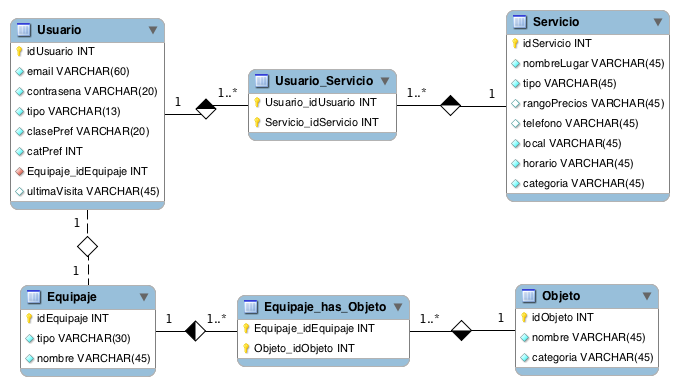
\includegraphics[width=0.8\textwidth]{Figuras/relacionalAdmin.png}
		\rule{30em}{0.5pt}
	\caption[Modelo Relacional de la Aplicación de Escritorio]{Modelo Relacional de la Aplicación de Escritorio}
	\label{fig:relacionalAdmin}
\end{figure}

\begin{figure}[h!]
	\centering
		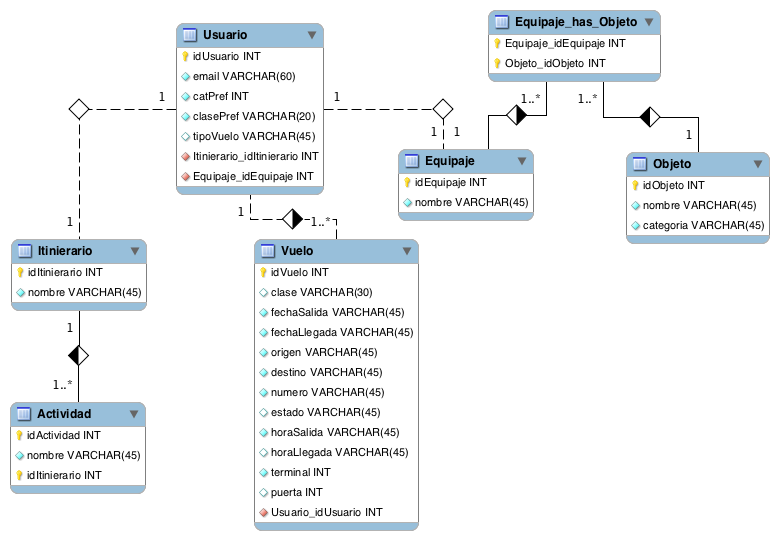
\includegraphics[width=1\textwidth]{Figuras/relacionalMovil.png}
		\rule{30em}{0.5pt}
	\caption[Modelo Relacional de la Aplicación Móvil]{Modelo Relacional de la Aplicación Móvil}
	\label{fig:relacionalMovil}
\end{figure}

En la Figura \ref{fig:relacionalTRASO} se muestra el modelo relacional de la base de datos que se realizó para el web service TRASO, que sustituyó a los servicios de Amadeus.

\begin{figure}[h!]
	\centering
		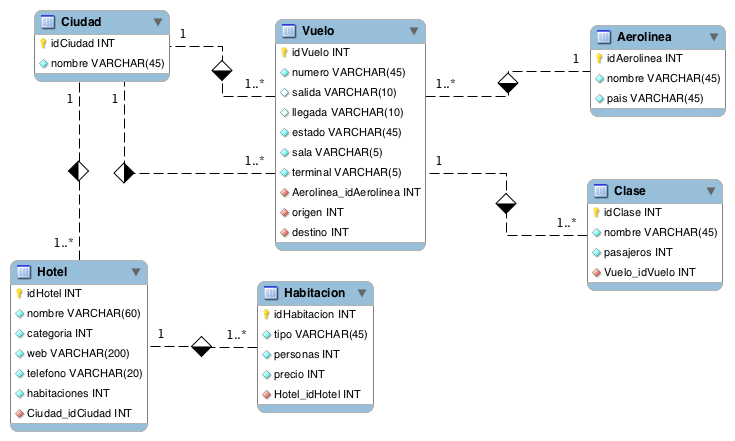
\includegraphics[width=0.8\textwidth]{Figuras/relacionalTRASO.png}
		\rule{30em}{0.5pt}
	\caption[Modelo Relacional del Web Service TRASO]{Modelo Relacional del Web Service TRASO}
	\label{fig:relacionalTRASO}
\end{figure}
\clearpage